\documentclass[10pt,a4paper]{article}
\usepackage[margin=1.5cm]{geometry}
\usepackage[T1]{fontenc}
\usepackage{graphicx,booktabs}
\usepackage[font=normalsize,labelfont=bf,skip=3pt]{caption}
\setlength{\parindent}{0pt}
\setlength{\parskip}{3pt}
\pagestyle{empty}
\newcommand{\h}[1]{\textbf{#1.}}
\renewcommand{\lg}{\log_2}

\begin{document}

\begin{center}
{\large\bfseries Skip List: Structural Union/Split and Experimental Analysis}
\end{center}
\vspace{-6pt}

\h{Design} A node is one heap block \texttt{\{key, height, next[height]\}}. The head is an array of 32 forward
pointers inside the list object and has no key, so every \texttt{int64\_t} (including \texttt{INT64\_MIN/MAX})
is a legal key; \texttt{nullptr} ends each level. Heights are geometric with $p=1/2$ (from the list's own
SplitMix64 generator, separate from the workload generator), capped at 32: for $n\le 2^{20}$ the chance
that any node is truncated is below $2.5\cdot10^{-4}$. A duplicate insert draws no height and changes nothing.
A list owns its nodes (movable, not copyable). \texttt{ordered\_union} and \texttt{split} relink the existing
nodes, keeping address, key and height, and leave their inputs empty and reusable. No size or tail pointer is stored.

\h{Expected costs} All bounds are expectations over the random heights, and with the height cap they are meant
for $n\le 2^{32}$ (not arbitrarily large $n$). Search/insert: the search path walked backwards climbs with
probability $1/2$ per step, so its expected length is $\le 2\lg n+O(1)$. Expected storage is $2n$ pointers.
\texttt{split} does one search to find the last node $\le x$ on each level, then cuts every level: expected
$O(\lg n)$. \texttt{ordered\_union} walks the right spine of $A$ and links $B$ after it on each level: expected
$O(\lg(n+m))$. The rebuilding baseline inserts every key into fresh lists: expected $\Theta(n\lg n)$ comparisons
and exactly $n$ allocations.

\h{Checks} An invariant checker verifies increasing keys per level, that level $i$ holds exactly the nodes of
height $>i$, valid links and no cycles. Results are compared with \texttt{std::set} on empty/singleton lists,
duplicates, boundary keys, split before/after/at a key, unequal or empty union inputs, \texttt{union(split(S,x))}
restoring $S$ with the same addresses and heights, independent outputs, reuse of consumed inputs, and 5\,000
mixed operations for each of 3 seeds: 82\,549 checks, 0 failures, also under AddressSanitizer + UBSan (no leaks).

\h{Method} Google Benchmark v1.8.3, GCC 11.4 \texttt{-O3}, WSL2 Ubuntu 22.04, AMD Ryzen AI 9 365, one thread.
$N=2^{10},2^{12},\dots,2^{20}$, 3 height seeds $\times$ 3 repetitions. Only the kernel is timed;
inputs are restored untimed; times are per operation. Search: 50\% hits. Insert: absent keys. Union:
$|A|=|B|=N/2$. Split: median pivot. Baseline: rebuilding split. Logical work (comparisons + link reads + writes)
and allocations come from a separate instrumented build on the same workloads (10 seeds).

\begin{figure}[h]
\centering
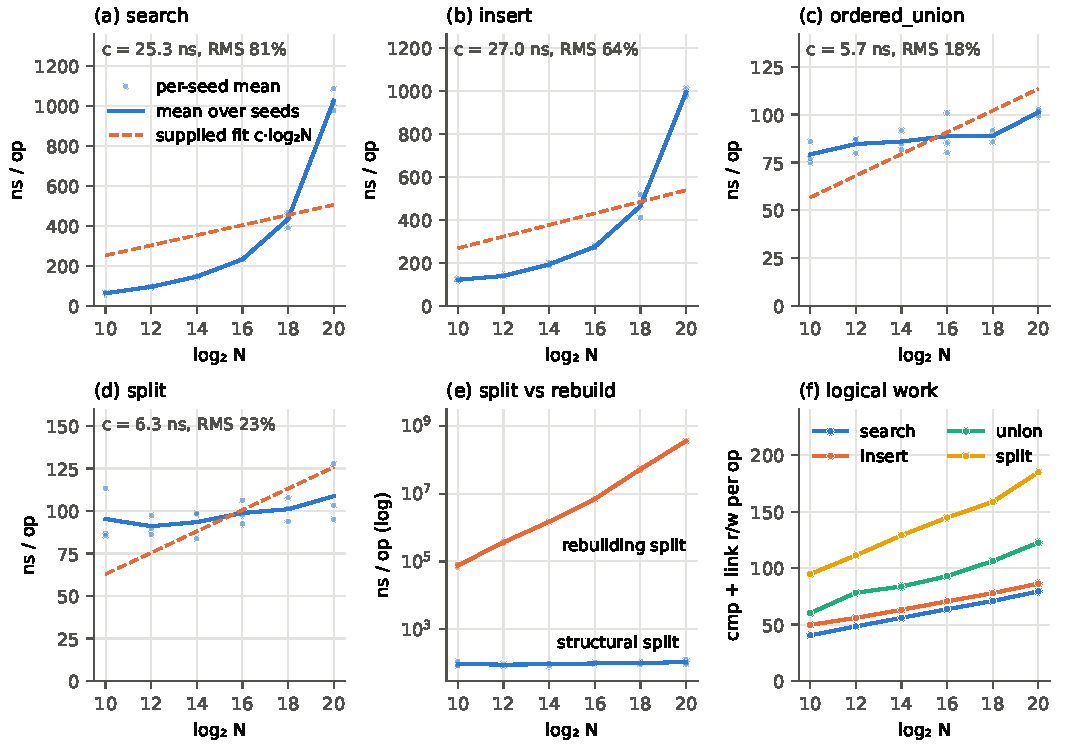
\includegraphics[width=\linewidth]{results/fig_scaling.pdf}
\caption{(a--d) time per operation (dots: per-seed means; dashed: fit $c\lg N$). (e) structural vs rebuilding split.
(f) logical work per operation from the instrumented build.}
\end{figure}
\h{Discussion} The logical work matches the analysis: search uses $1.97\lg N$ comparisons, and the total work of
all four kernels fits $c\lg N$ with at most 4\% RMS, with no allocations in the structural kernels. Search and insert
\emph{times} are not logarithmic here: from $2^{18}$ keys the list (about 40 MB at $2^{20}$) exceeds the 16\,MiB L3 cache and time per unit of work
rises from 1.6 to 13 ns; the $O(N)$ label reflects the memory hierarchy, not the operation count. Union and split are
nearly flat: each timed call retraces a path the untimed restoration just touched (cache-resident), and the 26\,ns
clock pair plus header handling dominate ${\approx}100$\,ns. The baseline does exactly $N$ allocations and frees and is
$8\cdot10^{2}\times$ slower than the structural split at $2^{10}$ and $3\cdot10^{6}\times$ at $2^{20}$; its time fits $N\lg N$ (Google Benchmark's own CPU-time choice is $N^2$, 19\%, almost as good), in line with its work, although time per
work unit rises from 2.2 to 5.4 ns once the data outgrows the caches.

\begin{center}
\begin{tabular}{lrrrr}
\toprule
 & ns/op, $2^{10}\!\to\!2^{20}$ & automatic fit (RMS) & $c\lg N$ fit (RMS) & work fit (RMS)\\
\midrule
search        & 64 $\to$ 1024 & $N$ (38\%)   & 25.3 (81\%) & $3.98\lg N$ (0.8\%)\\
insert        & 122 $\to$ 995 & $N$ (45\%)   & 27.0 (64\%) & $4.44\lg N$ (4.1\%)\\
union         & 79 $\to$ 101 & $1$ (12\%)   & 5.7 (18\%)  & $6.03\lg N$ (3.4\%)\\
split         & 95 $\to$ 109  & $1$ (16\%)   & 6.3 (23\%)  & $9.12\lg N$ (2.2\%)\\
split rebuild & $7.6\!\cdot\!10^4 \to 3.6\!\cdot\!10^8$ & $N\lg N$ (18\%) & -- & $3.17N\lg N$ (0.2\%)\\
\bottomrule
\end{tabular}

\captionof{table}{Fits on real time over all 54 runs (RMS normalised by the mean). Automatic fit: the best of Google
Benchmark's six models, re-selected on real time (Google Benchmark's own choice, made on CPU time, differs only
for split rebuild: $N^2$, 19\%); the $c\lg N$ model is our hypothesis.}
\end{center}

\h{Limitation} The structural timings are warm-cache and close to the timer overhead, so they cannot resolve the
logarithmic slope that the work counts show; WSL2 adds noise, and heights are capped at 32 ($n\le 2^{32}$).
A fitted model describes this size range, not asymptotic complexity (the $O(N)$ label does not mean the
algorithms are linear); the work counts support the expected $O(\lg n)$ targets.

\end{document}
